\chapter{The Length of Longest Literals}
\label{chap:length-of-longest-literals}

\pablo{Little introduction here, even if a bit repetitive. Also to introduce the symbols $u,v,$ etc}

Recall that in the BST-like model, $u$ is the probability of a concatenation node, $v$ is the probability of an alternation node, and $1-u-v$ is the probability of a Kleene star node. For a random regular expression tree of size $n$, the random variable $Y_n$ denotes the length of the longest literal extracted by Hyperscan, and we write $y_n=\EE[Y_n]$. This chapter studies the asymptotic behavior of $(y_n)$.

We first bound $(y_n)$ between deterministic recurrences. The upper bound replaces every maximum by a sum, while the lower bound uses the maximum of the expectations. The main deterministic object is the tightened lower bound $(z_n)$ defined in \eqref{eq:lower-bound-tighter}. We prove successively that $z_n=n^{\alpha+o(1)}$, that $z_n=\Theta(n^\alpha)$, and, under the stronger condition $u>1/2$, that $z_n\sim Cn^\alpha$ for some $C>0$; see Theorem~\ref{thm:exact-asymptotics}. The last section returns to the original stochastic recurrence and outlines a fixed-point approach for the asymptotics of $(y_n)$.

\section{Lower and upper bounds}

Consider the recurrence \eqref{eq:longest-literal-recurrence}. Denote $y_n := \EE[Y_n]$ for $n \ge 1$. Taking expectations in \eqref{eq:longest-literal-recurrence} gives, for $n \ge 1$,
\begin{equation}
  \label{eq:expected-longest-literal-recurrence}
  \begin{aligned}
    y_{n+2}
     & = \dfrac{u}{n}\sum\limits_{i=1}^n\left(y_{i} + y_{n+1-i}\right) + \dfrac{v}{n}\sum\limits_{i=1}^n\EE\left[\max\left(Y_{i}^{(1)}, Y_{n+1-i}^{(2)}\right)\right] \\
     & = \dfrac{2u}{n}\sum\limits_{i=1}^n y_{i} + \dfrac{v}{n}\sum\limits_{i=1}^n\EE\left[\max\left(Y_{i}^{(1)}, Y_{n+1-i}^{(2)}\right)\right].
  \end{aligned}
\end{equation}

Using the inequality $\max(a,b) \le a + b$ for $a,b \ge 0$, we have
$$y_{n+2} \le \dfrac{2(u+v)}{n}\sum\limits_{i=1}^n y_{i}.$$
Since the right-hand side of the inequality is an increasing function of $(y_1, \ldots, y_n)$, the sequence $(y_n)$ is bounded above by the solution to the recurrence
\begin{equation}
  \label{eq:upper-bound}
  z_{n+2} = \dfrac{2(u+v)}{n}\sum\limits_{i=1}^n z_{i}, \quad n \ge 1, \quad z_1 = 1, z_2 = 0.
\end{equation}
Similarly, the inequality $\max(a,b) \ge \frac{1}{2}(a+b)$ gives a lower bound sequence
\begin{equation}
  \label{eq:lower-bound}
  z_{n+2} = \dfrac{2u+v}{n}\sum\limits_{i=1}^n z_{i}, \quad n \ge 1, \quad z_1 = 1, z_2 = 0.
\end{equation}
A transfer theorem from analytic combinatorics gives the asymptotic behavior of \eqref{eq:upper-bound} and \eqref{eq:lower-bound}; see Appendix \ref{subsec:asymptotics-of-recurrences-that-include-a-sum-of-history}. The lower bound can be tightened by using
$$\EE\left[\max\left(Y_{i}^{(1)}, Y_{n+1-i}^{(2)}\right)\right] \ge \max\left(\EE\left[Y_{i}^{(1)}\right], \EE\left[Y_{n+1-i}^{(2)}\right]\right) = \max\left(y_i, y_{n+1-i}\right).$$
This is not sharp since equality holds only when $Y_{i}^{(1)} = Y_{n+1-i}^{(2)}$ a.s. The tightened lower bound recurrence is then given by
\begin{equation}
  \label{eq:lower-bound-tighter}
  z_{n+2} = \dfrac{2u}{n}\sum\limits_{i=1}^n z_{i} + \dfrac{v}{n}\sum\limits_{i=1}^n \max\left(z_i, z_{n+1-i}\right), \quad n \ge 1, \quad z_1 = 1, z_2 = 0.
\end{equation}
We analyze it in more detail in the next section.

\section{Asymptotics of the lower bound recurrence}

The sequence defined by \eqref{eq:lower-bound-tighter} is bounded between those defined by \eqref{eq:upper-bound} and \eqref{eq:lower-bound}. Under the conditions
\begin{equation}
  \label{eq:parameter-conditions}
  u,v \ge 0, \quad u < 1, \quad u+v\le1, \quad 2u+v > 1,
\end{equation}
both \eqref{eq:upper-bound} and \eqref{eq:lower-bound} grow as a pure power of $n$, without any lower-order factor such as a logarithm. In this section, we use several techniques to prove asymptotic theorems of increasing strength. The strongest theorem gives exact asymptotics, namely $z_n\sim Cn^{\alpha}$ for some constants $C > 0$ and $\alpha > 0$.

As a heuristic, assume that $z_n \sim Cn^{\alpha}$ for some constants $C > 0$ and $\alpha > 0$. Substituting this estimate into \eqref{eq:lower-bound-tighter}, we get
\begin{align*}
  Cn^\alpha
   & \sim \dfrac{2u}{n}\sum\limits_{i=1}^n C i^\alpha + \dfrac{v}{n}\sum\limits_{i=1}^n C\max\left(i^\alpha, (n+1-i)^\alpha\right)                   \\
   & \sim C\left( \dfrac{2u}{n}\int_0^n C x^\alpha\,\mathrm{d}x + \dfrac{v}{n}\int_0^n C\max\left(x^\alpha, (n-x)^\alpha\right) \,\mathrm{d}x\right) \\
   & = C\left(\dfrac{2u}{n}\int_0^n x^\alpha\,\mathrm{d}x + \dfrac{2v}{n}\cdot \int_{n/2}^{n} x^\alpha \,\mathrm{d}x\right)                          \\
   & = C\left(\dfrac{2u}{n}\cdot \dfrac{n^{\alpha+1}}{\alpha+1} + \dfrac{2v}{n}\cdot \dfrac{n^{\alpha+1}-(n/2)^{\alpha+1}}{\alpha+1}\right)          \\
   & = \dfrac{C}{\alpha+1}\left(2(u+v) - v2^{-\alpha}\right)n^{\alpha}.
\end{align*}
Thus, we must have
\begin{equation}
  \label{eq:alpha-equation}
  \alpha + v2^{-\alpha} = 2(u+v) - 1.
\end{equation}

The condition $2u+v>1$ ensures that $\alpha>0$; otherwise $2u+v = 1$. Numerical experiments regarding the ratio $z_n/n^{\alpha}$ are illustrated in Figure \ref{fig:ratios}. We now state the asymptotic theorems.

\begin{figure}
  \begin{subfigure}[c]{0.45\linewidth}
    \centering
    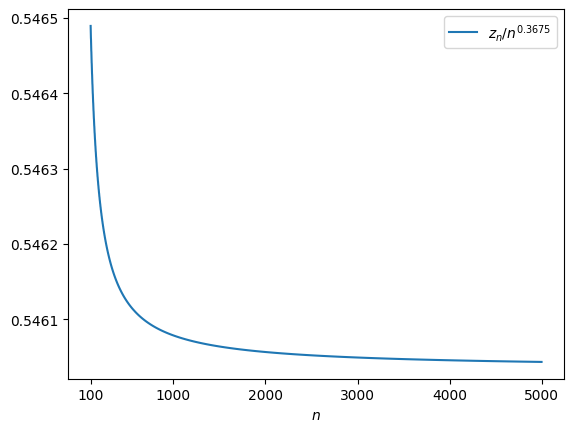
\includegraphics[width=\linewidth]{img/ratio-strict-lower-bound.png}
    \caption{Ratios $z_n/n^{\alpha}$ when $u = 0.5, v = 0.3$}
  \end{subfigure}
  \hfill
  \begin{subfigure}[c]{0.45\linewidth}
    \centering
    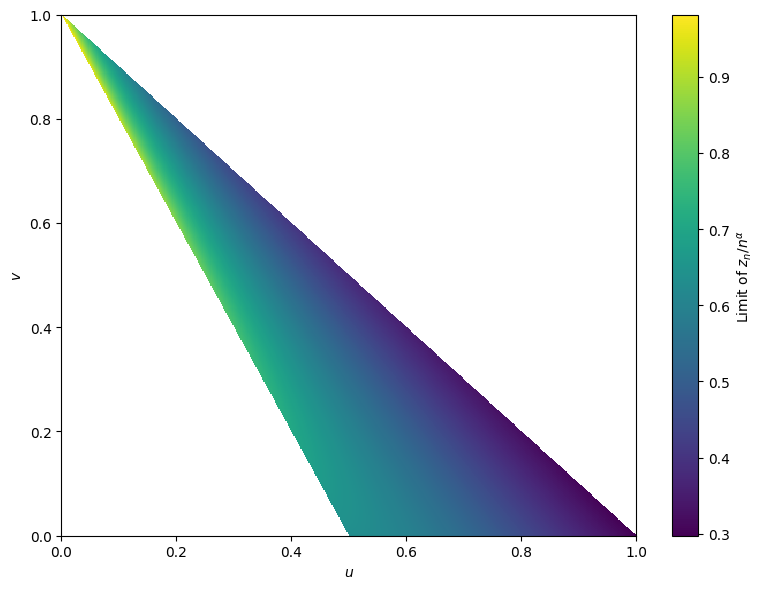
\includegraphics[width=\linewidth]{img/ratio-limits-strict-lower-bound.png}
    \caption{Limiting ratios for different $u$ and $v$.}
  \end{subfigure}

  \caption{Computation of $z_n/n^\alpha$}
  \label{fig:ratios}
\end{figure}


\begin{theorem}
  \label{thm:weaker-asymptotics}
  Let $\alpha$ be the solution to \eqref{eq:alpha-equation}. Then, $z_n = n^{\alpha + o(1)}$.
\end{theorem}

\begin{theorem}
  \label{thm:theta-asymptotics}
  Let $\alpha$ be the solution to \eqref{eq:alpha-equation}. Then, $z_n = \Theta(n^{\alpha})$.
\end{theorem}

For the exact asymptotics, we need to impose stricter conditions, for reasons that will become clear later.

\begin{equation}
  \label{eq:parameter-conditions-stronger}
  u,v \ge 0, \quad \dfrac{1}{2} < u < 1, \quad u+v\le1,
\end{equation}

\begin{theorem}
  \label{thm:exact-asymptotics}
  Let $(z_n)$ be defined by \eqref{eq:lower-bound-tighter}, let $\alpha$ be the solution to \eqref{eq:alpha-equation}, and let $u,v$ be the parameters satisfying \eqref{eq:parameter-conditions-stronger}. Then $z_n\sim C n^\alpha$ for some constant $C > 0$.
\end{theorem}

We begin with Theorem \ref{thm:weaker-asymptotics}. Rewrite the recurrence in \eqref{eq:lower-bound-tighter} as

\begin{equation}
  \label{eq:lower-bound-tighter-rewritten}
  z_{n+2} = \dfrac{1}{n}\sum\limits_{i=1}^n F(z_i, z_{n+1-i}), \quad n \ge 1,
\end{equation}
where
\begin{equation}
  F(x,y) = u(x+y) + v\max(x,y), \quad x,y > 0.
\end{equation}

Keeping in mind the heuristic $z_n \sim Cn^\alpha$, we try to approximate the right-hand side of \eqref{eq:lower-bound-tighter-rewritten}.

\begin{lemma}
  \label{thm:asymptoics-of-history}
  For every $\alpha \in (0,1]$, we have
  $$\dfrac{1}{n}\sum\limits_{i=1}^n F(i^\alpha, (n+1-i)^\alpha) \sim n^\alpha \Lambda(\alpha),$$
  where $\Lambda(\alpha) = \int_0^1 F(x^\alpha, (1-x)^\alpha) \,\mathrm{d}x = \dfrac{2(u+v)-v2^{-\alpha}}{\alpha+1}.$
\end{lemma}

\begin{proof}
  We will prove the equivalent limit
  $$\dfrac{1}{n}\sum\limits_{i=1}^n F\left(\left(\dfrac{i}{n}\right)^\alpha, \left(1-\dfrac{i}{n}+\dfrac{1}{n}\right)^\alpha\right) \to \Lambda(\alpha).$$

  Note that $\Lambda$ is continuous on $[0,1]$ with respect to $\alpha$, and the left-hand side is different from its Riemann sum only by a perturbation $1/n$ in the second argument. We show that the perturbation is negligible. Define for $x\in [0,1]$ the functions
  $$f_n(x) = F\left(x^\alpha, \left(1-x+\dfrac{1}{n}\right)^\alpha\right) \text{ and } f(x) = F(x^\alpha, (1-x)^\alpha).$$
  For $a,b,c \ge 0$ and $\alpha \in (0,1]$, we have
  $$|\max(a,b) - \max(a,c)| \le |b-c| \text{ and }
    (a+b)^\alpha \le a^\alpha + b^\alpha.$$
  Hence,
  \begin{align*}
    \|f_n-f\|_\infty
     & \le \sup\limits_{x\in[0,1]}(u+v)\left(\left(1-x+\dfrac{1}{n}\right)^\alpha - (1-x)^\alpha\right) \le (u+v)\dfrac{1}{n^\alpha} \to 0.
  \end{align*}

  Therefore,
  $$\left|\dfrac{1}{n}\sum\limits_{i=1}^n f_n\left(\dfrac{i}{n}\right) - \dfrac{1}{n}\sum\limits_{i=1}^n f\left(\dfrac{i}{n}\right)\right| \le \|f_n-f\|_\infty \to 0.$$
\end{proof}

The unique value of $\alpha$ such that $\Lambda(\alpha) = 1$ is the solution to \eqref{eq:alpha-equation}. To see this, compute
\begin{align*}
   & \Lambda'(\alpha) = \dfrac{v2^{-\alpha}\ln 2}{\alpha+1} - \dfrac{2(u+v)-v2^{-\alpha}}{(\alpha+1)^2} = \dfrac{v2^{-\alpha}((\alpha+1)\ln 2 + 1) - 2(u+v)}{(\alpha+1)^2}, \\
   & (2^{-\alpha}((\alpha+1)\ln 2 + 1))' = -2^{-\alpha}(\alpha+1)\ln^2(2) < 0.
\end{align*}
This implies
$$(\alpha+1)^2\Lambda'(\alpha) < (\alpha+1)^2\Lambda'(0) = -(2u + (1-\ln 2)v) < 0.$$
Hence, $\Lambda$ is strictly decreasing. We also have $\Lambda(0) = 2u+v > 1$ and $\Lambda(1) = u+v/2 < 1$. We exploit the fact that $\Lambda(\beta) > 1$ for $\beta < \alpha$ and $\Lambda(\beta) < 1$ for $\beta > \alpha$ to prove Theorem \ref{thm:weaker-asymptotics}.

\begin{proof}[Proof of Theorem \ref{thm:weaker-asymptotics}]
  Let $A_n(\beta) = \dfrac{1}{n}\sum\limits_{i=1}^n F(i^\beta, (n+1-i)^\beta)$. For the upper bound, let $\beta \in (\alpha, 1]$. Then $\Lambda(\beta) < 1$. Hence there exists $N$ such that for all $n \ge N$,
  $$A_n(\beta) < n^\beta < (n+2)^\beta.$$
  Let $M_n = \max_{1\le k \le n} \dfrac{z_i}{k^\beta}$. For $n \ge N$, we have
  $$z_{n+2} = \dfrac{1}{n}\sum_{i=1}^n F\left(z_i, z_{n+1-i}\right) \le M_n A_n(\beta) < M_n (n+2)^\beta.$$
  Hence, $\dfrac{z_{n+2}}{(n+2)^\beta} < M_n$. Thus $(M_n)$ is eventually decreasing, and $z_n = O(n^\beta)$.

  A similar argument applies for the lower bound, with an adjustment to deal with $z_2$. We have
  $$A_n(\beta) \sim n^\beta \sim (n+2)^\beta \text{ and } A_n(\beta) \sim \dfrac{1}{n}\sum\limits_{i=3}^{n-2} F(i^\beta, (n+1-i)^\beta).$$
  Assume that $\beta < \alpha$. Then, $\Lambda(\beta) > 1$. Hence there exists $N\ge 3$ such that for all $n \ge N$,
  $$\dfrac{1}{n}\sum\limits_{i=3}^{n-2} F(i^\beta, (n+1-i)^\beta) > (n+2)^\beta.$$
  Let $m_n = \min_{3\le i \le n-2} \dfrac{z_i}{i^\beta}$. For $n \ge N$, we have
  $$z_{n+2} \ge \dfrac{1}{n}\sum_{i=3}^{n-2} F\left(z_i, z_{n+1-i}\right) \ge m_n \dfrac{1}{n}\sum\limits_{i=3}^{n-2} F(i^\beta, (n+1-i)^\beta) > m_n (n+2)^\beta.$$
  Hence, $\dfrac{z_{n+2}}{(n+2)^\beta} > m_n$. Thus $(m_n)$ is eventually increasing, and $z_n = \Omega(n^\beta)$.
\end{proof}

The proof of Theorem \ref{thm:theta-asymptotics} uses a fine-grained induction. We first prepare integral bounds for the sum of the maximum terms.

\begin{lemma}
  \label{lem:integral-bounds}
  Let $f: [0, \infty) \to \mathbb{R}$ be an increasing function. For every integer $n \ge 1$, we have
  $$S_1 := \sum_{i=0}^{n-1} \max(f(i), f(n-1-i)) \le 2\int_{n/2}^n f(x) \, \mathrm{d}x \le S_2 :=\sum_{i=1}^{n} \max(f(i), f(n+1-i)). $$
\end{lemma}

\begin{proof}
  We first prove the upper bound on the first sum. We will use the following bounds for $t\ge 0$:
  $$f(t) \le \int_{t}^{t+1} f(x) \, \mathrm{d}x \le 2 \int_{t+1/2}^{t+1} f(x) \, \mathrm{d}x.$$

  If $n=2k$, we have
  $$S_1 = 2 \sum_{i=k}^{2k-1} f(i) \le 2 \sum_{i=k}^{2k-1} \int_{i}^{i+1} f(x) \, \mathrm{d}x.$$
  If $n=2k+1$, we have
  $$ S_1 = 2 \sum_{i=k+1}^{2k} f(i) + f(k) \le 2 \sum_{i=k+1}^{2k} \int_i^{i+1} f(x) \, \mathrm{d}x + 2 \int_{k+1/2}^{k+1} f(x) \, \mathrm{d}x.$$

  The lower bound on the second sum follows analogously from the following estimates. For $t\ge 1$, we have
  $$f(t) \ge \int_{t-1}^{t} f(x) \, \mathrm{d}x \ge 2 \int_{t-1}^{t-1/2} f(x) \, \mathrm{d}x.$$
\end{proof}


\begin{proof}[Proof of Theorem \ref{thm:theta-asymptotics}]
  We prove the lower bound. First, $z_n > 0$ for all $n\ne 2$. The main idea is to isolate $z_2$. The induction hypothesis is $z_n \ge K (n+L)^\alpha$ for $n\neq 2$. The base cases and the exact constants are determined later. We need
  $$\max(z_2, z_{n-1})= z_{n-1} \ge \max((2+L)^\alpha, (n-1+L)^\alpha).$$
  Thus, for $n \ge 3$,
  \begin{align*}
    nz_{n+2}
     & = 2u\sum\limits_{i=1}^n z_i + v\sum\limits_{i=1}^n \max(z_i, z_{n+1-i})                                                                \\
     & \ge K\left(2u\sum\limits_{i=1}^{n} (i+L)^\alpha + v\sum\limits_{i=1}^{n} \max((i+L)^\alpha, (n+1-i+L)^\alpha)\right) - K2u(2+L)^\alpha \\
     & \ge K\left(2u\int_0^{n} (x+L)^\alpha \, \mathrm{d}x + 2v\int_{n/2}^{n} (x+L)^\alpha \, \mathrm{d}x\right) - K2u(2+L)^\alpha.
  \end{align*}
  Let
  \begin{align*}
    A_n
     & = 2u\int_0^{n} (x+L)^\alpha \, \mathrm{d}x + 2v\int_{n/2}^{n} (x+L)^\alpha \, \mathrm{d}x             \\
     & = \dfrac{1}{\alpha+1}\left((2u+2v)(n+L)^{\alpha+1} - 2v\left(\dfrac{n}{2}+L\right)^{\alpha+1}\right).
  \end{align*}
  Using the expansions
  \begin{align*}
    (n+L)^{\alpha+1}                       & = n^{\alpha+1} + (\alpha+1)L n^\alpha + O(n^{\alpha-1}),                         \\
    \left(\dfrac{n}{2}+L\right)^{\alpha+1} & = 2^{-\alpha+1}n^{\alpha+1} + (\alpha+1)L2^{-\alpha} n^\alpha + O(n^{\alpha-1}),
  \end{align*}
  we get
  \begin{align*}
    A_n
     & = n^{\alpha+1} + L(2u+2v-2v2^{-\alpha})n^\alpha + O(n^{\alpha-1})        \\
     & = n^{\alpha+1} + L(\alpha + 1 - v2^{-\alpha})n^\alpha + O(n^{\alpha-1}).
  \end{align*}
  On the other hand,
  $$n(n+L+2)^\alpha = n^{\alpha+1} + \alpha(L+2) n^\alpha + O(n^{\alpha-1}).$$
  Hence,
  $$A_n - 2u(2+L)^\alpha - n(n+L+2)^\alpha = (L(1-v2^{-\alpha}) - 2\alpha) n^\alpha + O(n^{\alpha-1}).$$
  Since $1-v2^{-\alpha} > 0$, choose $L>\dfrac{2\alpha}{1-v2^{-\alpha}}$, then there exists $N$ such that for all $n \ge N$,
  $$A_n - 2u(2+L)^\alpha - n(n+L+2)^\alpha \ge 0,$$
  implying that $z_{n+2} \ge K(n+L+2)^\alpha$. Finally, we choose
  $$K = \min\limits_{\substack{1\le i\le N+1 \\ i\ne 2}}\dfrac{z_i}{(i+L)^\alpha} > 0$$
  to satisfy the base cases $i\le N+1$, excluding $i=2$ where $z_2=0$. \pablo{the base cases $i\leq N+1$ where $N$ is chosen to satisfy the above inequality.}

  \pablo{$K$ below is not the same as above. Write e.g., $\tilde{K}$}

  We now prove the upper bound. Our induction hypothesis is $z_n \le \tilde{K} (n-1)^\alpha$ for $n\ge 2$, for some constant $\tilde{K} > 1$. The base case $z_2=0$ is trivially satisfied. For $n\ge 2$, we have
  \begin{align*}
    nz_{n+2}
     & = 2u + 2u\sum\limits_{i=2}^n z_i + v\sum\limits_{i=1}^n \max(z_i, z_{n+1-i})                                              \\
     & \le \tilde{K}\left(2u\sum\limits_{i=1}^{n-1} i^\alpha + v\sum\limits_{i=0}^{n-1} \max(i^\alpha, (n-1-i)^\alpha)\right)+2u \\
     & \le \tilde{K}\left(2u\int_1^{n} x^\alpha \, \mathrm{d}x + 2v\int_{n/2}^{n} x^\alpha \, \mathrm{d}x\right) + 2u            \\
     & = \tilde{K}\left(2u\dfrac{n^{\alpha+1} - 1}{\alpha+1} + 2v\dfrac{n^{\alpha+1} - (n/2)^{\alpha+1}}{\alpha+1}\right)+2u     \\
     & = \tilde{K}n^{\alpha+1}\dfrac{2u+2v - v2^{-\alpha}}{\alpha+1}- \dfrac{2\tilde{K}u}{\alpha+1}+2u                           \\
     & = \tilde{K}n^{\alpha+1} - \dfrac{2\tilde{K}u}{\alpha+1} + 2u.
  \end{align*}


  The first inequality is valid by noticing that
  $$\max(z_1, z_n) = \max(1, z_n) \le \tilde{K}(n-1)^\alpha = \tilde{K}\max(0, (n-1)^\alpha).$$
  The second inequality uses Lemma \ref{lem:integral-bounds}. Choose $\tilde{K}=\alpha+1 > 1$, then $z_{n+2} \le \tilde{K}n^\alpha \le \tilde{K}(n+2)^\alpha$.
\end{proof}

\begin{remark}
  In the proof of the lower bound, we use the fact that $(n+L)^{\alpha+1}$ dominates $n(n+L+2)^{\alpha+1}$ when $L$ is large enough. Similarly, $(n-L)^{\alpha+1} \ll n(n-L+2)^{\alpha+1}$ for large $L$. However, applying the same idea to the upper bound would start the induction only after some $n > L$. We avoid this by choosing $L=1$ and saving a fixed budget $2u$ in the first term, which also gives a useful algebraic simplification.
\end{remark}

We now prove the exact asymptotics stated in Theorem \ref{thm:exact-asymptotics}. A natural goal is to remove the maximum operator. If $z_1=z_2=1$, then the sequence would be increasing from the beginning, and induction would allow us to eliminate the maximum operator. However, the initial conditions $z_1=1$ and $z_2=0$ make the sequence $(z_n)$ fluctuate during the first iterations, and the index at which it becomes increasing depends on the parameters $u$ and $v$. An extreme case of a long fluctuation period occurs when $u\to1/2+$ and $v\to0+$. We illustrate this phenomenon and compare the two cases in Figure~\ref{fig:difference-beginning}. The figure compares the consecutive differences of the same recurrence under two close initializations, $z_1=z_2=1$ and $z_1=1,z_2=0$, in the difficult regime $u=0.5000001$ and $v=0.000001$. The second initialization can create a long initial fluctuation, which explains why monotonicity cannot simply be assumed from the beginning.

\begin{figure}
  \begin{subfigure}[c]{0.45\linewidth}
    \centering
    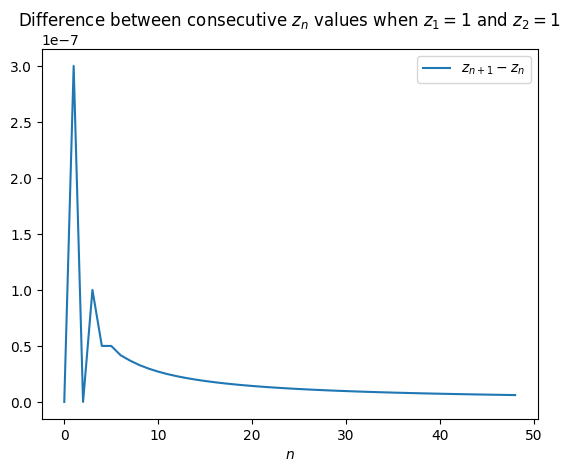
\includegraphics[width=\linewidth]{img/strict-lower-bound-11.png}
  \end{subfigure}
  \hfill
  \begin{subfigure}[c]{0.45\linewidth}
    \centering
    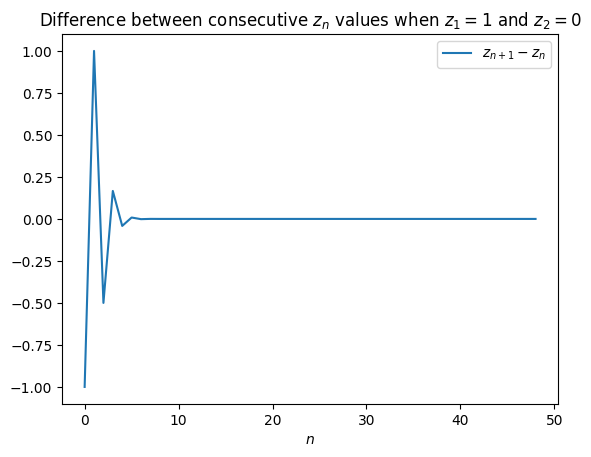
\includegraphics[width=\linewidth]{img/strict-lower-bound-10.png}
  \end{subfigure}

  \caption{First consecutive differences of $(z_n)$ in two initializations ($u = 0.5000001, v = 0.000001$)}
  \label{fig:difference-beginning}
\end{figure}

\pablo{Give experimental examples.}



Eventual monotonicity is sufficient to remove the maximum operator. Assume that there exists $N_1$ such that $z_{n+1} \ge z_n$ for all $n \ge N_1$. Since $(z_n)$ is unbounded, there exists $N_2 \ge N_1$ such that for all $n \ge N_2$, we have both $z_{n+1} \ge \max\limits_{1\le i \le N_1} z_i$ and $z_{n+1} \ge z_n$. That is,
$$\forall n \ge N_2, \quad z_{n+1} \ge \max_{1 \le i \le n} z_i.$$
Taking $N_3 = 2N_2-1$, we have \cyril{the writing $\forall \dfrac{N_3+1}{2}\le i \le N_3$ looks weird}
$$\forall n \ge N_3,\quad \forall i\in\left\{\left\lceil\dfrac{n+1}{2}\right\rceil,\ldots,n\right\}, \quad z_{i} \ge z_{n+1-i}.$$

Under the stronger parameter condition \eqref{eq:parameter-conditions-stronger}, Theorem~\ref{thm:eventually-increasing} below proves that such an index exists. The question about the first index where the fluctuations stop is itself interesting, and we leave it open.
\begin{openquestion}
  \label{open:when-eventually-increasing}
  In terms of $u$ and $v$, what is the first index $N$ such that $(z_n)_{n\ge N}$ is increasing?
\end{openquestion}


\pablo{The existence of $N$  is Theorem~\ref{thm:eventually-increasing}, right ? You can announce the results, otherwise one might think that the existence of $N$ is conjectured.}

We proceed to proving eventual monotonicity. The idea is to use loose inequalities to bootstrap basic properties, then upgrade step by step with tighter inequalities. The next lemma uses a loose inequality $\max(a,b)\le a+b$ to show that the difference between consecutive terms vanishes. To begin with, let us define for $n\ge 1$ the difference
$$\Delta z_n = z_{n} - z_{n-1}.$$

\begin{lemma}[Vanishing difference]
  \label{lem:vanishing-difference}
  We have $|\Delta z_n| \to 0$.
\end{lemma}

\begin{proof}
  For $n \ge 2$, we have
  \begin{align*}
    nz_{n+2}     & = 2u\sum_{i=1}^n z_i + v\sum_{i=1}^n \max(z_i, z_{n+1-i}),       \\
    (n-1)z_{n+1} & = 2u\sum_{i=1}^{n-1} z_i + v\sum_{i=1}^{n-1} \max(z_i, z_{n-i}).
  \end{align*}
  Subtracting the equations side by side, we get
  \begin{equation}
    \label{eq:difference}
    \begin{aligned}
      n\Delta z_{n+2}
       & = 2uz_n + v\max(z_n,z_1) - z_{n+1} + v\sum_{i=1}^{n-1} (\max(z_i, z_{n+1-i}) - \max(z_i, z_{n-i}))      \\
       & = 2uz_n + v\max(z_n,z_1) - z_{n+1} + v\sum_{i=1}^{n-1} (\max(z_{n-i}, z_{i+1}) - \max(z_{n-i}, z_{i})).
    \end{aligned}
  \end{equation}
  Using $\max(z_n, z_1) \le z_n+z_1$, we have
  \begin{align*}
    n\Delta z_{n+2}
     & \le 2uz_n + v(z_n + z_1) - vz_{n+1} + v\sum_{i=1}^{n-1} (\max(z_{n-i}, z_{i+1}) - \max(z_{n-i}, z_{i})) \\
     & \le 2uz_n + vz_1 + v(z_n - z_{n+1}) + v\sum_{i=1}^{n-1} (\max(z_{n-i}, z_{i+1}) - \max(z_{n-i}, z_{i}))
  \end{align*}
  Using $|\max(a,b) - \max(a,c)| \le |b-c|$, we have
  \begin{align*}
    n|\Delta z_{n+2}|
     & \le 2uz_n + vz_1 + v|\Delta z_n| + v\sum_{i=1}^{n-1} |\Delta z_i| = 2uz_n + vz_1 + v\sum_{i=1}^{n}|\Delta z_i| \\
     & \le 2uz_n + vz_1 + nv\sup_{1\le i \le n}|\Delta z_i|.
  \end{align*}
  Since $u < 1$, we have $\alpha < 1$. By $z_n = \Theta(n^\alpha)$, we have $\dfrac{1}{n}(2uz_n + vz_1) \to 0$, or
  $$|\Delta z_{n+2}| \le v\sup_{1\le i \le n}|\Delta z_i| + o(1).$$
  We have $v < 1$ since otherwise the condition $2u+v > 1$ would be violated. Therefore $(|\Delta z_i|)$ is bounded. Let $M = \sup_{n \ge 1} |\Delta z_n|$. For every $\epsilon > 0$, there exists $N$ such that for all $n \ge N$, $|\Delta z_n| < M + \epsilon$. Therefore,
  $$|\Delta z_{n+2}| \le v(M+\epsilon) + o(1).$$
  Letting $n\to\infty$ gives $M \le v(M+\epsilon)$. Since $\epsilon > 0$ is arbitrary, we have $M = 0$.
\end{proof}

Since $(z_n)$ is unbounded, we have the following corollary.

\begin{corollary}[Eventual exceedance]
  \label{cor:eventual-exceed}
  Let $\alpha$ be the solution to \eqref{eq:alpha-equation}. Then, for every $M > 0$, there exists $N$ such that for all $n \ge N$, $z_n > M$.
\end{corollary}

\begin{lemma}[Difference identity]
  \label{lem:difference-identity}
  For all sufficiently large $n$, there exist numbers $\theta_{n,i}\in [0,1]$ for $1\le i\le n-1$ such that
  \begin{equation}
    \label{eq:difference-identity}
    n\Delta z_{n+2} = (2u+v-1)z_n-\Delta z_n +v\sum_{i=1}^{n-1}\theta_{n,i}\Delta z_i.
  \end{equation}
\end{lemma}

\begin{proof}
  We start from \eqref{eq:difference}
  $$n\Delta z_{n+2} = 2uz_n + v\max(z_n,z_1) - z_{n+2} + v\sum_{i=1}^{n-1} (\max(z_i, z_{n+2-i}) - \max(z_i, z_{n-i})).$$
  By Corollary \ref{cor:eventual-exceed}, we have $\max(z_n,z_1)=z_n$ for all sufficiently large $n$. Hence, for all sufficiently large $n$,
  $$n\Delta z_{n+2} = (2u+v-1)z_n -\Delta z_n + v\sum_{i=1}^{n-1} (\max(z_{n-i}, z_{i+2}) - \max(z_{n-i}, z_{i})).$$
  For every $a \ge 0$, the function $x\mapsto \max(a,x)$ is increasing and $1$-Lipschitz. Hence for each $n,i$ there is some $\theta_{n,i}\in[0,1]$ satisfying \eqref{eq:difference-identity}.
\end{proof}

At this step, we have isolated the difference sequence $(\Delta z_n)$ from the original sequence $(z_n)$. Our next goal is to prove that $(\Delta z_n)$ is \textit{eventually positive}. This would follow if, in \eqref{eq:difference-identity}, a lower bound for $-\Delta z_n + v\sum_{i=1}^{n-1}\theta_{n,i}\Delta z_i$ could be absorbed into $(2u+v-1)z_n$. We already have $|\Delta z_n| = o(z_n)$ since $(\Delta z_n)$ is bounded.

Because little is known about $\theta_{n,i}$, we can only use a worst-case bound. A basic absolute-value estimate would require proving that $\sum_{i=1}^{n}|\Delta z_i| = o(z_n)$. However, if $z_n\sim Cn^\alpha$ and $z_n$ is eventually increasing, then $\sum_{i=1}^{n}|\Delta z_i| \sim Cn^\alpha$. We therefore need a tighter lower bound. We use the \textit{negative variation} of $\Delta z_n$, defined for every $x\in\mathbb{R}$ as
\begin{equation}
  x_{-} = \max(-x,0).
\end{equation}

We have
\begin{equation}
  \label{ineq:negative-variation}
  -x \le x_{-} \text{ and } 0 \le x_{-}.
\end{equation}

Define the negative variation series of $(\Delta z_n)$ as
\begin{equation}
  \label{eq:negative-variation}
  V_n := \sum_{i=1}^{n} (\Delta z_i)_{-}.
\end{equation}
Then $(V_n)$ is increasing. We state the criterion for eventual increase of $(z_n)$ in terms of $(V_n)$ as follows.

\begin{lemma}[Negative variation criterion]
  If $V_n = o(z_n)$, then $(z_n)$ is eventually increasing.
\end{lemma}

\begin{proof}
  By Lemma~\ref{lem:difference-identity}, for all sufficiently large $n$,
  $$n\Delta z_{n+2} \ge (2u+v-1)z_n-|\Delta z_n|-vV_n.$$
  Since $\Delta z_n$ is bounded and $z_n\to\infty$, we have $|\Delta z_n|=o(z_n)$. By assumption, $V_n = o(z_n)$. Hence for all sufficiently large $n$,
  $$n\Delta z_{n+2} \ge \dfrac{1}{2}(2u+v-1)z_n > 0$$
\end{proof}

% It would be perfect if we could prove that $(V_n)$ is bounded, as this is indeed the truth. However, it is already good to prove that $V_n = o(n^\alpha)$, since we already have $z_n = \Theta(n^\alpha)$.

\pablo{``probably'' or ``likely' ' rather than ``indeed''}

Numerical experiments suggest that $(V_n)$ is likely bounded. For the proof of eventual monotonicity, however, the following weaker estimate is enough.

\begin{lemma}
  Assume that $v>0$.
  We have $V_n = O(n^v)$.
\end{lemma}

\begin{proof}
  Again, we start from \eqref{eq:difference-identity}. There exists $N$ such that for all $n\ge N$,
  $$n\Delta z_{n+2} = (2u+v-1)z_n - \Delta z_n + v\sum_{j=1}^{n-1}\theta_{n,j}\Delta z_j.$$
  Let $M = \sup |\Delta z_n|$. \pablo{You mean $\Delta z_n$. Also, I am not convinced of the next equality. You do have the inequality with $v \sum (\Delta z_j)_-$, but not an equality as it is not true that $(x+y)_-=x_-+y_-$}
  If $\Delta z_{n+2}\ge 0$, then $(\Delta z_{n+2})_- = 0$. Otherwise, $(\Delta z_{n+2})_- = -\Delta z_{n+2}$, and therefore
  \begin{align*}
    n(\Delta z_{n+2})_-
     & = \Delta z_n - (2u+v-1)z_n - v\sum_{j=1}^{n-1}\theta_{n,j}\Delta z_j                                                       \\
     & \le |\Delta z_n| - (2u+v-1)z_n + v\sum_{j=1}^{n-1}\theta_{n,j}(\Delta z_j)_- & (- \Delta z_j\le (\Delta z_j)_-, \forall j) \\
     & \le |\Delta z_n| + v\sum_{j=1}^{n-1}(\Delta z_j)_-                           & (0\le\theta_{n,j}\le1)                      \\
     & \le M + vV_{n-1}.
  \end{align*}
  Thus, in either case,
  $$(\Delta z_{n+2})_- \le \dfrac{v}{n}V_{n-1}+\dfrac{M}{n}.$$
  Since $(V_n)$ is increasing, we get
  \begin{equation}
    \label{eq:negative-variation-bound}
    V_{n+2}
    = V_{n+1}+(\Delta z_{n+2})_-
    \le \left(1+\dfrac{v}{n}\right)V_{n+1}+\dfrac{M}{n}.
  \end{equation}
  Reindexing, for every $m\ge N+2$,
  $$V_m + \dfrac{M}{v} \le \left(1+\dfrac{v}{m-2}\right)\left(V_{m-1} + \dfrac{M}{v}\right).$$
  Iterating this inequality gives
  $$V_m + \dfrac{M}{v}
    \le \prod_{i=N}^{m-2}\left(1+\dfrac{v}{i}\right)\left(V_{N+1} + \dfrac{M}{v}\right).$$
  It remains to estimate the product. Taking the logarithm gives
  \begin{align*}
    \ln\left(\prod_{i=N}^{m-2}\left(1+\frac{v}{i}\right) \right)
     & = \sum_{i=N}^{m-2}\ln\left(1+\frac{v}{i}\right)         \\
     & \le \sum_{i=N}^{m-2} \frac{v}{i} = v(H_{m-2} - H_{N-1}) \\
     & \le vH_m \le v\ln m + C,
  \end{align*}
  where $H_n=\sum_{i=1}^n \frac{1}{i} = \ln n + \gamma + O(1/n)$ is the $n$-th harmonic number and $C$ is some constant. Exponentiating both sides yields
  $$\prod_{i=N}^{m-2} \left( 1 + \frac{v}{i} \right) \le e^{C} m^v = O(m^v).$$
\end{proof}

We state our checkpoint as a theorem.

\begin{theorem}
  \label{thm:eventually-increasing}
  If $0<v < \alpha$, then $(z_n)$ is eventually increasing.
\end{theorem}

\begin{proof}
  By the previous lemma, $V_n=O(n^v)=o(n^\alpha)=o(z_n)$, since $v<\alpha$ and $z_n=\Theta(n^\alpha)$. The result follows from the negative variation criterion.
\end{proof}

When $v=0$, the recurrence \eqref{eq:lower-bound-tighter} reduces to the full-history recurrence \eqref{eq:lower-bound}, whose asymptotics are handled by Proposition~\ref{lem:full-history-sum-asymptotics}. Thus the negative-variation argument is only needed for $v>0$.

We now express the condition $0<v < \alpha$ in terms of $u$ and $v$. Define
$$f(\alpha) = \alpha + 1 - 2(u + v) + v 2^{-\alpha}, \alpha\in[0,1].$$
Then $f'(\alpha) = 1 - v2^{-\alpha}\ln2 > 1-\ln2 > 0$ for all $\alpha > 0$. Hence $v < \alpha$ is equivalent to $f(v) < 0$ i.e.,
$$v + 1 - 2(u + v) + v 2^{-v} < 0 \iff u > \frac{1}{2}(1 - v + v 2^{-v}).$$
For $v>0$, if we impose conditions \eqref{eq:parameter-conditions-stronger}, then the above inequality is satisfied. The case $v\ge \alpha$ with $v>0$ is left open. Once $(z_n)$ is eventually increasing, it satisfies a simpler recurrence without the whole history.

\begin{lemma}
  There exists $N\ge 1$ such that the sequence $(z_n)_{n\ge N}$ defined by \ref{eq:lower-bound-tighter} satisfies the recurrence
  \begin{equation}
    \label{eq:delayed-recurrence}
    nz_{n+2}-(n-1)z_{n+1} = 2(u+v)z_{n} - vz_{\lfloor n/2\rfloor}.
  \end{equation}
  with $z_{N+1} \ge z_{N} \ge \ldots \ge z_{\lfloor n/2\rfloor} \ge 1$.
\end{lemma}

\begin{proof}
  Since $(z_n)$ is eventually increasing, there exists $N$ such that for all $n\ge N$, we have $z_n \ge z_i$ for all $1\le i \le n-1$ and $z_n \ge 1$. Hence, for all $n\ge N+1$,
  \begin{align*}
    nz_{n+2}     & = 2u\sum_{i=1}^n z_i + 2v\sum_{i=\lceil n/2\rceil+1}^n z_i + \delta_nvz_{\lceil n/2\rceil}                      \\
    (n-1)z_{n+1} & = 2u\sum_{i=1}^{n-1} z_i + 2v\sum_{i=\lceil (n-1)/2\rceil+1}^{n-1} z_i + \delta_{n-1}vz_{\lceil (n-1)/2\rceil},
  \end{align*}
  where $\delta_n = 1$ if $n$ is odd and $0$ if $n$ is even. If $n=2k$, then $\lceil n/2\rceil = \lceil (n-1)/2\rceil = k$, $\delta_n = 0$ and $\delta_{n-1} = 1$. Hence,
  $$2kz_{2k+2} - (2k-1)z_{2k+1} = 2(u+v)z_{2k} - vz_{k}.$$
  If $n=2k+1$, then $\lceil n/2\rceil > \lceil (n-1)/2\rceil = k$, $\delta_n = 1$ and $\delta_{n-1} = 0$. Hence,
  $$(2k+1)z_{2k+3} - (2k)z_{2k+2} = 2(u+v)z_{2k+1} - 2vz_{k+1} + vz_{k+1} = (2k+1)(u+v)z_{2k+1} - vz_{k+1}.$$
  Collecting the two cases and noticing that $\left\lceil\dfrac{n-1}{2}\right\rceil = \left\lfloor\dfrac{n}{2}\right\rfloor$, we arrive at \eqref{eq:delayed-recurrence}.
\end{proof}

With the recurrence \eqref{eq:delayed-recurrence}, we can now prove the exact asymptotics of $(z_n)$. We will use a dyadic argument to show that the normalized difference sequence $(\Delta x_n)$ is absolutely summable by analyzing it on the intervals $[2^m, 2^{m+1})$.

        \pablo{You can pre-state this result at the beginning of the chapter to outline it, citing it forward.}

        \begin{proof}[Proof of Theorem~\ref{thm:exact-asymptotics}]
          Let $x_n=\dfrac{z_n}{(n-2)^\alpha}$ for $n\ge N$. We will prove that $(x_n)$ converges by proving that $(\Delta x_n)$ is absolutely summable, i.e., $\sum_{n\ge N}|\Delta x_n|$ converges. Note that $x_n = \Theta(1)$ since $z_n = \Theta(n^\alpha)$. For $n\ge N \ge 6$ (so that $x_{\lfloor n/2\rfloor}$ is defined), we have
          \begin{align*}
                 & n^{\alpha+1} x_{n+2} - (n-1)^{\alpha+1} x_{n+1} = 2(u+v)(n-2)^{\alpha}x_{n} - v\left(\left\lfloor \dfrac{n}{2}\right\rfloor-2\right)^{\alpha}x_{\lfloor n/2\rfloor}                                               \\
            \iff & x_{n+2} = \left(1-\dfrac{1}{n}\right)^{\alpha+1}x_{n+1} + \dfrac{2(u+v)}{n}\left(1-\dfrac{2}{n}\right)^{\alpha}x_{n-1} - \dfrac{v}{n}\left(\dfrac{\lfloor n/2\rfloor-2}{n}\right)^{\alpha}x_{\lfloor n/2\rfloor}.
          \end{align*}
          We have
          \begin{align*}
             & \left(1-\dfrac{1}{n}\right)^{\alpha+1} = 1 - \dfrac{\alpha+1}{n} + O\left(\dfrac{1}{n^2}\right),                        \\
             & \dfrac{1}{n}\left(1-\dfrac{2}{n}\right)^{\alpha} = \dfrac{1}{n} + O\left(\dfrac{1}{n^2}\right),                         \\
             & \frac{1}{n}\left(\dfrac{\lfloor n/2\rfloor-2}{n}\right)^{\alpha} = \frac{2^{-\alpha}}{n} + O\left(\frac{1}{n^2}\right).
          \end{align*}
          The last expansion follows from $\dfrac{1}{2}-\dfrac{3}{n} \le \dfrac{\lfloor n/2\rfloor-2}{n} \le \dfrac{1}{2}-\dfrac{1}{n}$. Since $\alpha$ solves \eqref{eq:alpha-equation}, we have
          \begin{align*}
            x_{n+2}-x_{n+1}
             & = -\dfrac{\alpha+1}{n}x_{n+1} + \dfrac{2(u+v)}{n}x_{n} - \frac{v2^{-\alpha}}{n}x_{\lfloor n/2\rfloor} + O\left(\frac{1}{n^2}\right)   \\
             & = -\dfrac{2(u+v)}{n}(x_{n+1}-x_{n}) + \frac{v2^{-\alpha}}{n}\left(x_{n}- x_{\lfloor n/2\rfloor}\right) + O\left(\frac{1}{n^2}\right).
          \end{align*}

          There exists a constant $K_1>0$ such that for every $n\ge N'-2 \ge N$,
          $$|\Delta x_{n+2}| \le \dfrac{2(u+v)}{n}|\Delta x_{n+1}| + \frac{v2^{-\alpha}}{n}\sum_{i=\lfloor n/2\rfloor + 1}^{n}|\Delta x_{i}| + \dfrac{K_1}{(n+2)^2}.$$
          Equivalently, for $n\ge N'$,
          $$|\Delta x_{n}| \le \dfrac{2(u+v)}{n-2}|\Delta x_{n-1}| + \frac{v2^{-\alpha}}{n-2}\sum_{i=\lfloor n/2\rfloor}^{n-2}|\Delta x_{i}| + \dfrac{K_1}{n^2}.$$

          Let $u_m = \max_{2^m \le n < 2^{m+1}} |\Delta x_n|$. Then, for every $n\in [2^m, 2^{m+1})$, we have
          \begin{align*}
             & |\Delta x_{n-1}| \le \max_{2^m-1\le i < 2^{m+1}-1}|\Delta x_i| \le \max(u_{m-1},u_m),                                                                             \\
             & \dfrac{1}{n-2}\sum_{i=\lfloor n/2\rfloor}^{n-2}|\Delta x_{i}| \le \dfrac{1}{2}\max_{2^{m-1}\le i < 2^{m+1}-2} |\Delta x_i|\le  \dfrac{1}{2} \max(u_{m-1}, u_{m}).
          \end{align*}
          Therefore,
          \begin{align*}
            |\Delta x_{n}|
             & \le \left(\dfrac{2(u+v)}{n-2}+v2^{-\alpha-1}\right)\max(u_{m-1},u_m) + \dfrac{K_1}{2^{2m}}.
          \end{align*}
          Taking the maximum over $n\in [2^m, 2^{m+1})$, we have
          \begin{align*}
            u_m
             & \le \left(\dfrac{2(u+v)}{n-2}+v2^{-\alpha-1}\right)\max(u_{m-1},u_m) + \dfrac{K_1}{2^{2m}}.
          \end{align*}
          Since $v2^{-\alpha} = 2(u+v)-\alpha-1 < 1$, we can choose $m_0$ large enough such that $2^{m_0} \ge N'$, and there exists $\gamma_1$ such that
          $$\dfrac{2(u+v)}{n-2}+ v2^{-\alpha-1} < \gamma_1 < \dfrac{1}{2}$$
          for all $m\ge m_0$ and $n\in [2^m, 2^{m+1})$. If $u_{m-1} > u_m$, then $u_m \le \gamma_1 u_{m-1} + \dfrac{K_1}{2^{2m}}$. If $u_{m-1} \le u_m$, then $u_m \le \dfrac{K_1}{2^{2m}(1-\gamma_1)}$. In both cases, we have
          \begin{align*}
            u_m
             & \le \gamma_1 u_{m-1} + \dfrac{K_1}{2^{2m}(1-\gamma_1)}                                                             \\
             & \le \sum_{i=m_0+1}^m \gamma_1^{m-i}\dfrac{K_1}{2^{2i}(1-\gamma_1)} + \gamma_1^{m-m_0}u_{m_0}                       \\
             & < \dfrac{K_1}{(1-\gamma_1)}\sum_{i=m_0+1}^m \gamma_1^{m-i}\left(\dfrac{1}{4}\right)^{i} + \gamma_1^{m-m_0}u_{m_0}.
          \end{align*}
          Choose $\gamma_2$ such that $\max\left(\gamma_1, \dfrac{1}{4}\right) < \gamma_2 < \dfrac{1}{2}$. We have
          \begin{align*}
            u_m < \dfrac{K_1}{(1-\gamma_1)}\sum_{i=m_0+1}^m \gamma_2^m + \gamma_2^{m-m_0}u_{m_0} \le K_2 m\gamma_2^m,
          \end{align*}
          for some constant $K_2>0$. Choose $\gamma_3$ such that $\gamma_2 < \gamma_3 < \dfrac{1}{2}$. Then there exists $m_1>m_0$ such that for every $m\ge m_1$, we have $K_2m\gamma_2^m < K_2\gamma_3^m$, implying that
          $$u_m < K_2\gamma_3^m.$$
          Therefore,
          \begin{align*}
            \sum_{n=N'+1}^\infty|\Delta x_{m}|
             & \le \sum_{m=\lfloor\log_2(N')\rfloor}^\infty \sum_{n=2^m}^{2^{m+1}-1}|\Delta x_n| < \sum_{m=\lfloor\log_2(N')\rfloor}^{m_1-1} 2^m u_m  + K_2\sum_{m=m_1}^\infty (2\gamma_3)^{m} < \infty.
          \end{align*}
          Hence, $(x_n)$ converges to some constant $C>0$. Thus, $z_n \sim Cn^\alpha$.
        \end{proof}

        \section{Asymptotics of the stochastic recurrence}

        \subsection{Proof strategy}

        The stochastic recurrence \eqref{eq:longest-literal-recurrence} resembles its deterministic counterpart \eqref{eq:lower-bound-tighter}. Since \eqref{eq:lower-bound-tighter} grows as a pure power of $n$, it is natural to conjecture the same behavior for the expectation in \eqref{eq:expected-longest-literal-recurrence}. Numerical experiments based on Monte Carlo simulation support this conjecture, as shown in Figure \ref{fig:growth-comparison}. For each case of $(u,v)$, we compute the exponent $\alpha$ using the algorithm expressed in \eqref{eq:mean-preserving-recurrence}, and the constant $C=z_n/n^\alpha$, where $n$ is the number of iterations. More details of the algorithm are given later in this section.

        The growth exponent of $y_n$ is strictly larger than the solution to \eqref{eq:alpha-equation}. This suggests that, in the long term, $\EE\left[\max(Y_i, Y_j)\right]$ remains more selective than $\max(\EE[Y_i], \EE[Y_j])$, especially when $i$ and $j$ are close to each other.

        \begin{figure}
          \begin{subfigure}[c]{0.45\linewidth}
            \centering
            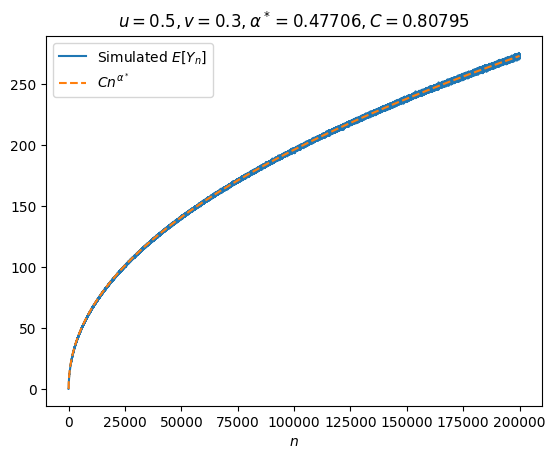
\includegraphics[width=\linewidth]{img/05-03-100000-200000.png}
          \end{subfigure}
          \hfill
          \begin{subfigure}[c]{0.45\linewidth}
            \centering
            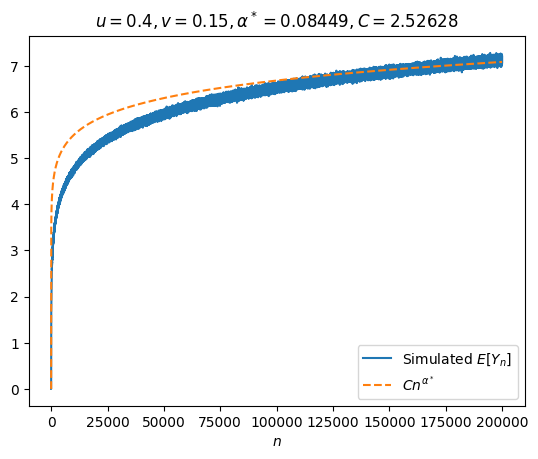
\includegraphics[width=\linewidth]{img/04-015-100000-200000.png}
          \end{subfigure}

          \caption{The growth of $y_n$ compared with a power $Cn^\alpha$}
          \label{fig:growth-comparison}
        \end{figure}


        In this section, we present an ongoing attempt to prove the weakest asymptotic result $y_n = n^{\alpha^\star + o(1)}$. We adapt the contraction method (e.g., \cite{neininger2004general}). The original idea is as follows.
        \begin{enumerate}
          \item Guess the scaling factor and derive the normalized recurrence.
          \item Derive a limiting fixed-point equation from the normalized recurrence.
          \item Prove that the limiting equation has a unique solution in a suitable metric space using a contraction argument.
          \item Prove that the normalized sequence converges in distribution to that unique solution.
        \end{enumerate}

        We first explain why the contraction method does not apply directly. Let $X_n = Y_n/n^\alpha$ for $\alpha > 0$. The recurrence for $X_n$ and the limiting equation are as follows.

        \begin{equation}
          \label{eq:scaled-recurrence}
          \begin{aligned}
            X_{n+2}
             & \stackrel{d}{=} I\left(\left(\dfrac{U_n}{n+2}\right)^\alpha X_{U_n}^{(1)} + \left(\dfrac{n+1-U_n}{n+2}\right)^\alpha X_{n+1-U_n}^{(2)}\right)   \\
             & \myspace{50} + J\max\left(\left(\dfrac{U_n}{n+2}\right)^\alpha X_{U_n}^{(1)}, \left(\dfrac{n+1-U_n}{n+2}\right)^\alpha X_{n+1-U_n}^{(2)}\right)
          \end{aligned}
        \end{equation}

        \begin{lemma}[Limiting equation]
          \label{lem:limiting-equation}
          Suppose that $X_n \stackrel{d}{\to} X$. Then, $X$ satisfies the following distributional equation
          \begin{equation}
            \label{eq:limiting-equation}
            X \stackrel{d}{=} I\left(U^\alpha X^{(1)} + (1-U)^\alpha X^{(2)}\right) + J\max(U^\alpha X^{(1)}, (1-U)^\alpha X^{(2)}),
          \end{equation}
          where $U \sim \mathrm{Unif}[0,1]$.
        \end{lemma}

        The proof of Lemma \ref{lem:limiting-equation} is given in Appendix \ref{subsec:proof-limiting-equation}. Let $\D$ be the space of probability measures on $\mathbb{R}_+$. Our first goal is to prove that there exists a unique solution $(X^\star,\alpha^\star)$ to \eqref{eq:limiting-equation} in some subspace of $\D$. The fixed-point equation \eqref{eq:limiting-equation} always has a degenerate solution $\delta_0$. The question is therefore to choose a suitable subspace that excludes $\delta_0$. Define the operator $T_\alpha: \D \to \D$ induced by the right-hand side of \eqref{eq:limiting-equation} as
        \begin{equation}
          \label{eq:operator-T}
          T_{\alpha}(\mu) = \mathcal{L}\left(I\left(U^\alpha X^{(1)} + (1-U)^\alpha X^{(2)}\right) + J\max(U^\alpha X^{(1)}, (1-U)^\alpha X^{(2)})\right), \quad X^{(1)}, X^{(2)} \stackrel{\text{iid}}{\sim}\mu.
        \end{equation}
        If $T_\alpha$ is a contraction with respect to the Wasserstein metric for some $\alpha$, then the Banach fixed-point theorem guarantees that $T^n_\alpha(\mu_1) \xrightarrow{d} 0$. While the Zolotarev metric \cite{zolotarev1977approximation} allows us to choose a subspace excluding $\delta_0$, it requires certain first moments to remain fixed---a condition $T_\alpha$ violates, as it does not preserve the mean. The original contraction method requires choosing a more suitable metric space, which we consider intractable.

        The evolution of an initial distribution under $T_\alpha$ can be understood as follows. At each iteration, $T_\alpha$ changes the shape of the distribution $\mu_n$. Depending on the ``dispersion'' of $\mu_n$, $T_\alpha$ either increases or decreases its mean. If $\alpha$ is too large, $T_\alpha$ drives the mean to $0$ before the distribution becomes sufficiently dispersed. Conversely, if $\alpha$ is too small, $T_\alpha$ pushes the mean to infinity once the distribution is sufficiently dispersed.

        The mean is not positively correlated with the need for a larger $\alpha$. Let $\mu = \delta_2$ and $\nu = 2\text{Ber}(1/2)$, so that $\EE_{X\sim\mu}[X] = 2 > 1 = \EE_{Y\sim\nu}[Y]$. If $\alpha$ solves \eqref{eq:alpha-equation}, then $\EE_{X\sim\mu}[T_\alpha(X)] = \EE_{X\sim\mu}[X]$, but $\EE_{Y\sim\nu}[T_\alpha(Y)] > \EE_{Y\sim\nu}[Y]$. Thus, although $\mu$ has a larger mean than $\nu$, it requires a smaller $\alpha$ to keep its mean fixed. This is because $\nu$ is more dispersed than $\mu$.

        The second moment is still not sufficient. One can build a similar counterexample by choosing $\mu$ and $\nu$ with the same mean, $\mathbb{E}_{X\sim\mu}[X^2] > \mathbb{E}_{Y\sim\nu}[Y^2]$, and $\mathbb{E}_{X\sim\mu}[X^3] < \mathbb{E}_{Y\sim\nu}[Y^3]$. If the third moments differ enough compared with the second moments, then $\EE_{X\sim\mu}[T_\alpha(X)] < \EE_{Y\sim\nu}[T_\alpha(Y)]$. Thus no finite number of moments is sufficient to determine the correct $\alpha$ that keeps the mean fixed.

        For each distribution $\mu$ of finite mean, there exists a unique $\alpha$ that keeps the mean fixed. Since $T_\alpha$ is homogeneous, we consider the space $\D(1)$ of probability measures on $\mathbb{R}_+$ with mean $1$. We state the property below and leave the proof to Appendix \ref{subsec:proof-prop-f}.

        \begin{proposition}
          \label{prop:f}
          Define the function $f: \D(1)\times(0,1] \to \RR_+$ as
          $$f(\mu, \alpha) = \EE_{Y\sim T_\alpha(\mu)}[X] = \dfrac{2u}{\alpha+1} + v \EE_{X^{(1)}, X^{(2)}\sim\mu}\left[\max\left(U^\alpha X^{(1)}, (1-U)^\alpha X^{(2)}\right)\right].$$

          For every $\mu\in \D_2(1)$, there exists a unique $\alpha\in[\alpha_0, 2(u+v)-1)$, where $\alpha_0$ solves \eqref{eq:alpha-equation}, such that $f(\mu, \alpha) = 1$. Moreover, the range is sharp:
          $$\forall \alpha \in (0,\alpha_0), f(\mu, \alpha) > 1 \text{ and } \forall \epsilon\in (0,2u+v-1-\alpha_0), \exists \mu\in \D_2(1), f(\mu, \alpha) = 1.$$
        \end{proposition}

        A promising approach for finding the true $\alpha$ is to let the distribution and its mean-preserving operator evolve together. By Proposition \ref{prop:f}, the function $\alpha: \mathcal{D}(1) \to (0,1]$ such that $\EE_{X\sim\mu}[T_{\alpha(\mu)}(X)] = 1$ is well-defined. We can then define the mean-preserving recurrence as follows.

\begin{equation}
  \label{eq:mean-preserving-recurrence}
  \mu_{n+1} = T_{\alpha_n}(\mu_n), \,\,\, \alpha_{n} = \alpha(\mu_{n}) \quad\quad \mu_1 = \delta_1, \,\,\, \alpha_1 = \alpha(\mu_1).
\end{equation}

\begin{figure}
  \begin{subfigure}[c]{0.45\linewidth}
    \centering
    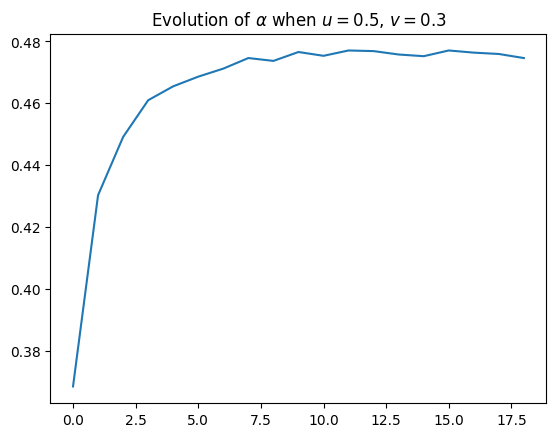
\includegraphics[width=\linewidth]{img/alpha-evolution.png}
    \caption{The evolution of $\alpha_n$}
  \end{subfigure}
  \hfill
  \begin{subfigure}[c]{0.45\linewidth}
    \centering
    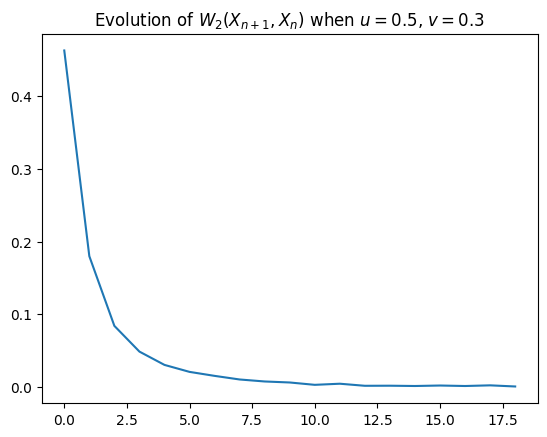
\includegraphics[width=\linewidth]{img/w2-evolution.png}
    \caption{The evolution of $W_2(\mu_{n+1}, \mu_n)$}
  \end{subfigure}

  \caption{Results of the mean-preserving recurrence \eqref{eq:mean-preserving-recurrence} with $u=0.5$ and $v=0.3$}
  \label{fig:mean-preserving-recurrence-evolution}
\end{figure}

The evolution of $\alpha$ and the 2-Wasserstein distance between consecutive distributions following the recurrence is shown in Figure \ref{fig:mean-preserving-recurrence-evolution}. Fluctuations in the final iterations are likely a side effect of the Monte Carlo simulation, since they become more stable when the number of samples is increased. However, proving that $(\mu_n, \alpha_n)$ converges may be challenging. We intended to track a quantity that evolves monotonically with the iterations. Experiments suggest in particular that the higher moments increase through iterations, but we could not complete this approach. Our alternative strategy takes advantage of Tychonoff's theorem, a non-constructive topological existence result. We summarize our proof strategy as follows, and proceed with the first step in the next subsection.
\begin{enumerate}
  \item Prove that there exists a unique solution $(X^\star, \alpha^\star)$ to \eqref{eq:limiting-equation}.
  \item Prove that for every $\epsilon > 0$, $\EE\left[Y_n/n^{\alpha^\star + \epsilon}\right]\to 0$ and $\EE\left[Y_n/n^{\alpha^\star - \epsilon}\right]\to \infty$.
  \item Prove that \eqref{eq:mean-preserving-recurrence} converges to $(X^\star, \alpha^\star)$.
\end{enumerate}

In the next subsection, we present a partial result towards the first step.

\subsection{A fixed-point approach: existence}

Since the contraction argument may not be applicable to proving uniqueness of the fixed point, we decompose the problem into proving existence and then uniqueness. Existence is proved using Tychonoff's fixed-point theorem.

\begin{theorem}[{Tychonoff \cite[Exercise 2.5c]{zeidler1986nonlinear}}]
  Let $\C$ be a nonempty, compact, convex subset of a locally convex space $\M$. Let $f: \C \to \C$ be a continuous mapping. Then $f$ has a fixed point.
\end{theorem}

We now prepare the ingredients for the Tychonoff fixed-point theorem. Ideally, the subset $\C$ should be as small as possible while still containing $(\mu_n)$ in \eqref{eq:mean-preserving-recurrence} and $(\L(X_n))$ for $X_n$ defined in \eqref{eq:scaled-recurrence} for all $\alpha\in(2u+v-1, 2u+v)$. This makes uniqueness more plausible once existence is established. Define $\Phi: \D(1) \to \D(1)$ by
\begin{equation}
  \label{eq:operator-phi}
  \Phi(\mu) = T_{\alpha(\mu)}(\mu), \quad \forall \mu\in \D(1).
\end{equation}

In the following, we will show that the subset $\C$ can be restricted to the set of distributions with uniformly bounded second moment. For $M > 0$, define
\begin{equation}
  \label{eq:bounded-second-moment}
  \D_2(1, M) = \left\{\mu\in \D(1): \int_{0}^\infty x^2 \,\mathrm{d}\mu \le M\right\}.
\end{equation}

\begin{proposition}
  \label{prop:uniform-bounded-second-moment}
  Assume that $u>1/2$. Then there exists $M_0 > 0$ such that for every $M \ge M_0 $, the operator $\Phi$ defined in \eqref{eq:operator-phi} maps $\D_2(1, M)$ into itself.
\end{proposition}


The proof is given in Appendix \ref{subsec:proof-prop-phi}. Again, the condition $u>1/2$ is crucial. Choose $M = \max(1, M_0)$. In $D_2(1,M)$, the range in Proposition \ref{prop:f} can be slightly improved to $\left[\alpha_0, 2(u+v)-1-\dfrac{v}{2M}\right)$.

The next ingredient is the host vector space $\M$. To avoid excessive elaboration, we combine two standard points of view. From probability theory, weak convergence can be defined using the space $C_b(\RR)$ of bounded, continuous test functions \cite[Chap. 1]{billingsley1999convergence}. From functional analysis, local convexity is obtained by equipping $C_b(\RR)$ with a topology and defining $\M$ as its dual space of continuous linear functionals. In this way, the weak topology on $\M$ (called the weak$^*$-topology in functional analysis) is induced by a family of seminorms $\{p_f\}_{f\in C_b(\RR)}$, which makes $\M$ a locally convex space. Finally, it is enough to have $\D_2(1, M)$ compact in $\M$. However, just as we want $\D_2(1, M)$ to be only large enough to contain our distributions of interest, we also want $\M$ to be only large enough to contain $\D_2(1, M)$, since a smaller host space is usually better behaved. We summarize the above discussion as follows, leaving the details to Appendix \ref{subsec:supp-locally-convex-spaces} and Appendix \ref{subsec:proof-prop-phi-continuity}.

\begin{theorem}[{Dual space of $C_b(\RR)$ with the strict topology \cite{buck1958bounded}}]
  \label{thm:dual-strict-topology}
  Equip $C_b(\RR)$ with the strict topology. Then the dual space is isometrically isomorphic to the space $\M(\RR)$ of bounded Radon measures on $\RR$. Moreover, $\M(\RR)$ is locally convex with respect to the weak topology.
\end{theorem}

\begin{proposition}
  \label{prop:nonempty-compact-convex}
  The set $\D_2(1, M)$ is a nonempty, compact, and convex subset of the space $\M(\RR)$ defined in Theorem \ref{thm:dual-strict-topology}.
\end{proposition}

\begin{proposition}
  \label{prop:phi-continuity}
  The operator $\Phi$ defined in \eqref{eq:operator-phi} is continuous on $\D_2(1, M)$ with respect to the weak topology.
\end{proposition}

A useful property of $\D_2(1, M)$ is that for any $\mu \in \D_2(1, M)$ and any $R > 0$, by Chebyshev's inequality, we have
$$\int_{R}^\infty x \,\mathrm{d}\mu \le \int_{R}^\infty x \left(\frac{x}{R} \right) \mathrm{d}\mu = \frac{1}{R} \int_{R}^\infty x^2 \,\mathrm{d}\mu \le \frac{1}{R} \int_{0}^\infty x^2 \,\mathrm{d}\mu \le \frac{M}{R}.$$
This implies tightness and uniform integrability of $\D_2(1, M)$. Tightness is used in proving compactness, and uniform integrability is used in proving continuity of $\Phi$ by identifying weak continuity with $W_1$-continuity.

These ingredients allow us to apply Tychonoff's fixed-point theorem.

\begin{theorem}
  \label{thm:existence-fixed-point}
  Assume that $u > 1/2$. Then there exists a solution
  $$(\mu^\star, \alpha^\star)\in \D_2(1, M)\times\left[\alpha_0, 2(u+v)-1-\dfrac{v}{2M}\right),$$
  where $\alpha_0$ solves \eqref{eq:alpha-equation}, to the fixed-point equation \eqref{eq:limiting-equation}.
\end{theorem}

% \textcolor{red}{We could construct $(\mu^\star, \alpha^\star)$. Are we really using nonconstructive topological tools somewhere?}

% \textcolor{red}{Is $\D(1)$ compact in $\M$?}



% \begin{remark}
%   If we relax the condition that the second moment is uniformly bounded.
% \end{remark}



% The problems of stronger asymptotic results remain open. Another interesting question left open is follows.

% \begin{openquestion}
%   \label{openq:alpha-algebraic}
%   Given that $y_n = n^{\alpha^\star + o(1)}$, is there an algebraic equation for $\alpha^\star$?
% \end{openquestion}
